\section{Homepage}
Volendo fare un paragone con il mondo fisico, possiamo considerare un sito web come l'alter-ego virtuale di un negozio (e, nel caso di un e-commerce come MyProtein, direi che non c'è metafora più azzeccata). L'amo del negozio fisico è la vetrina, che possiamo far corrispondere alla \textbf{homepage}: il suo compito è quello di catturare l'utente, far sì che prosegua la navigazione (ovvero entri nel negozio) e magari acquisti anche qualcosa.
\begin{figure}[!htb]
	\center{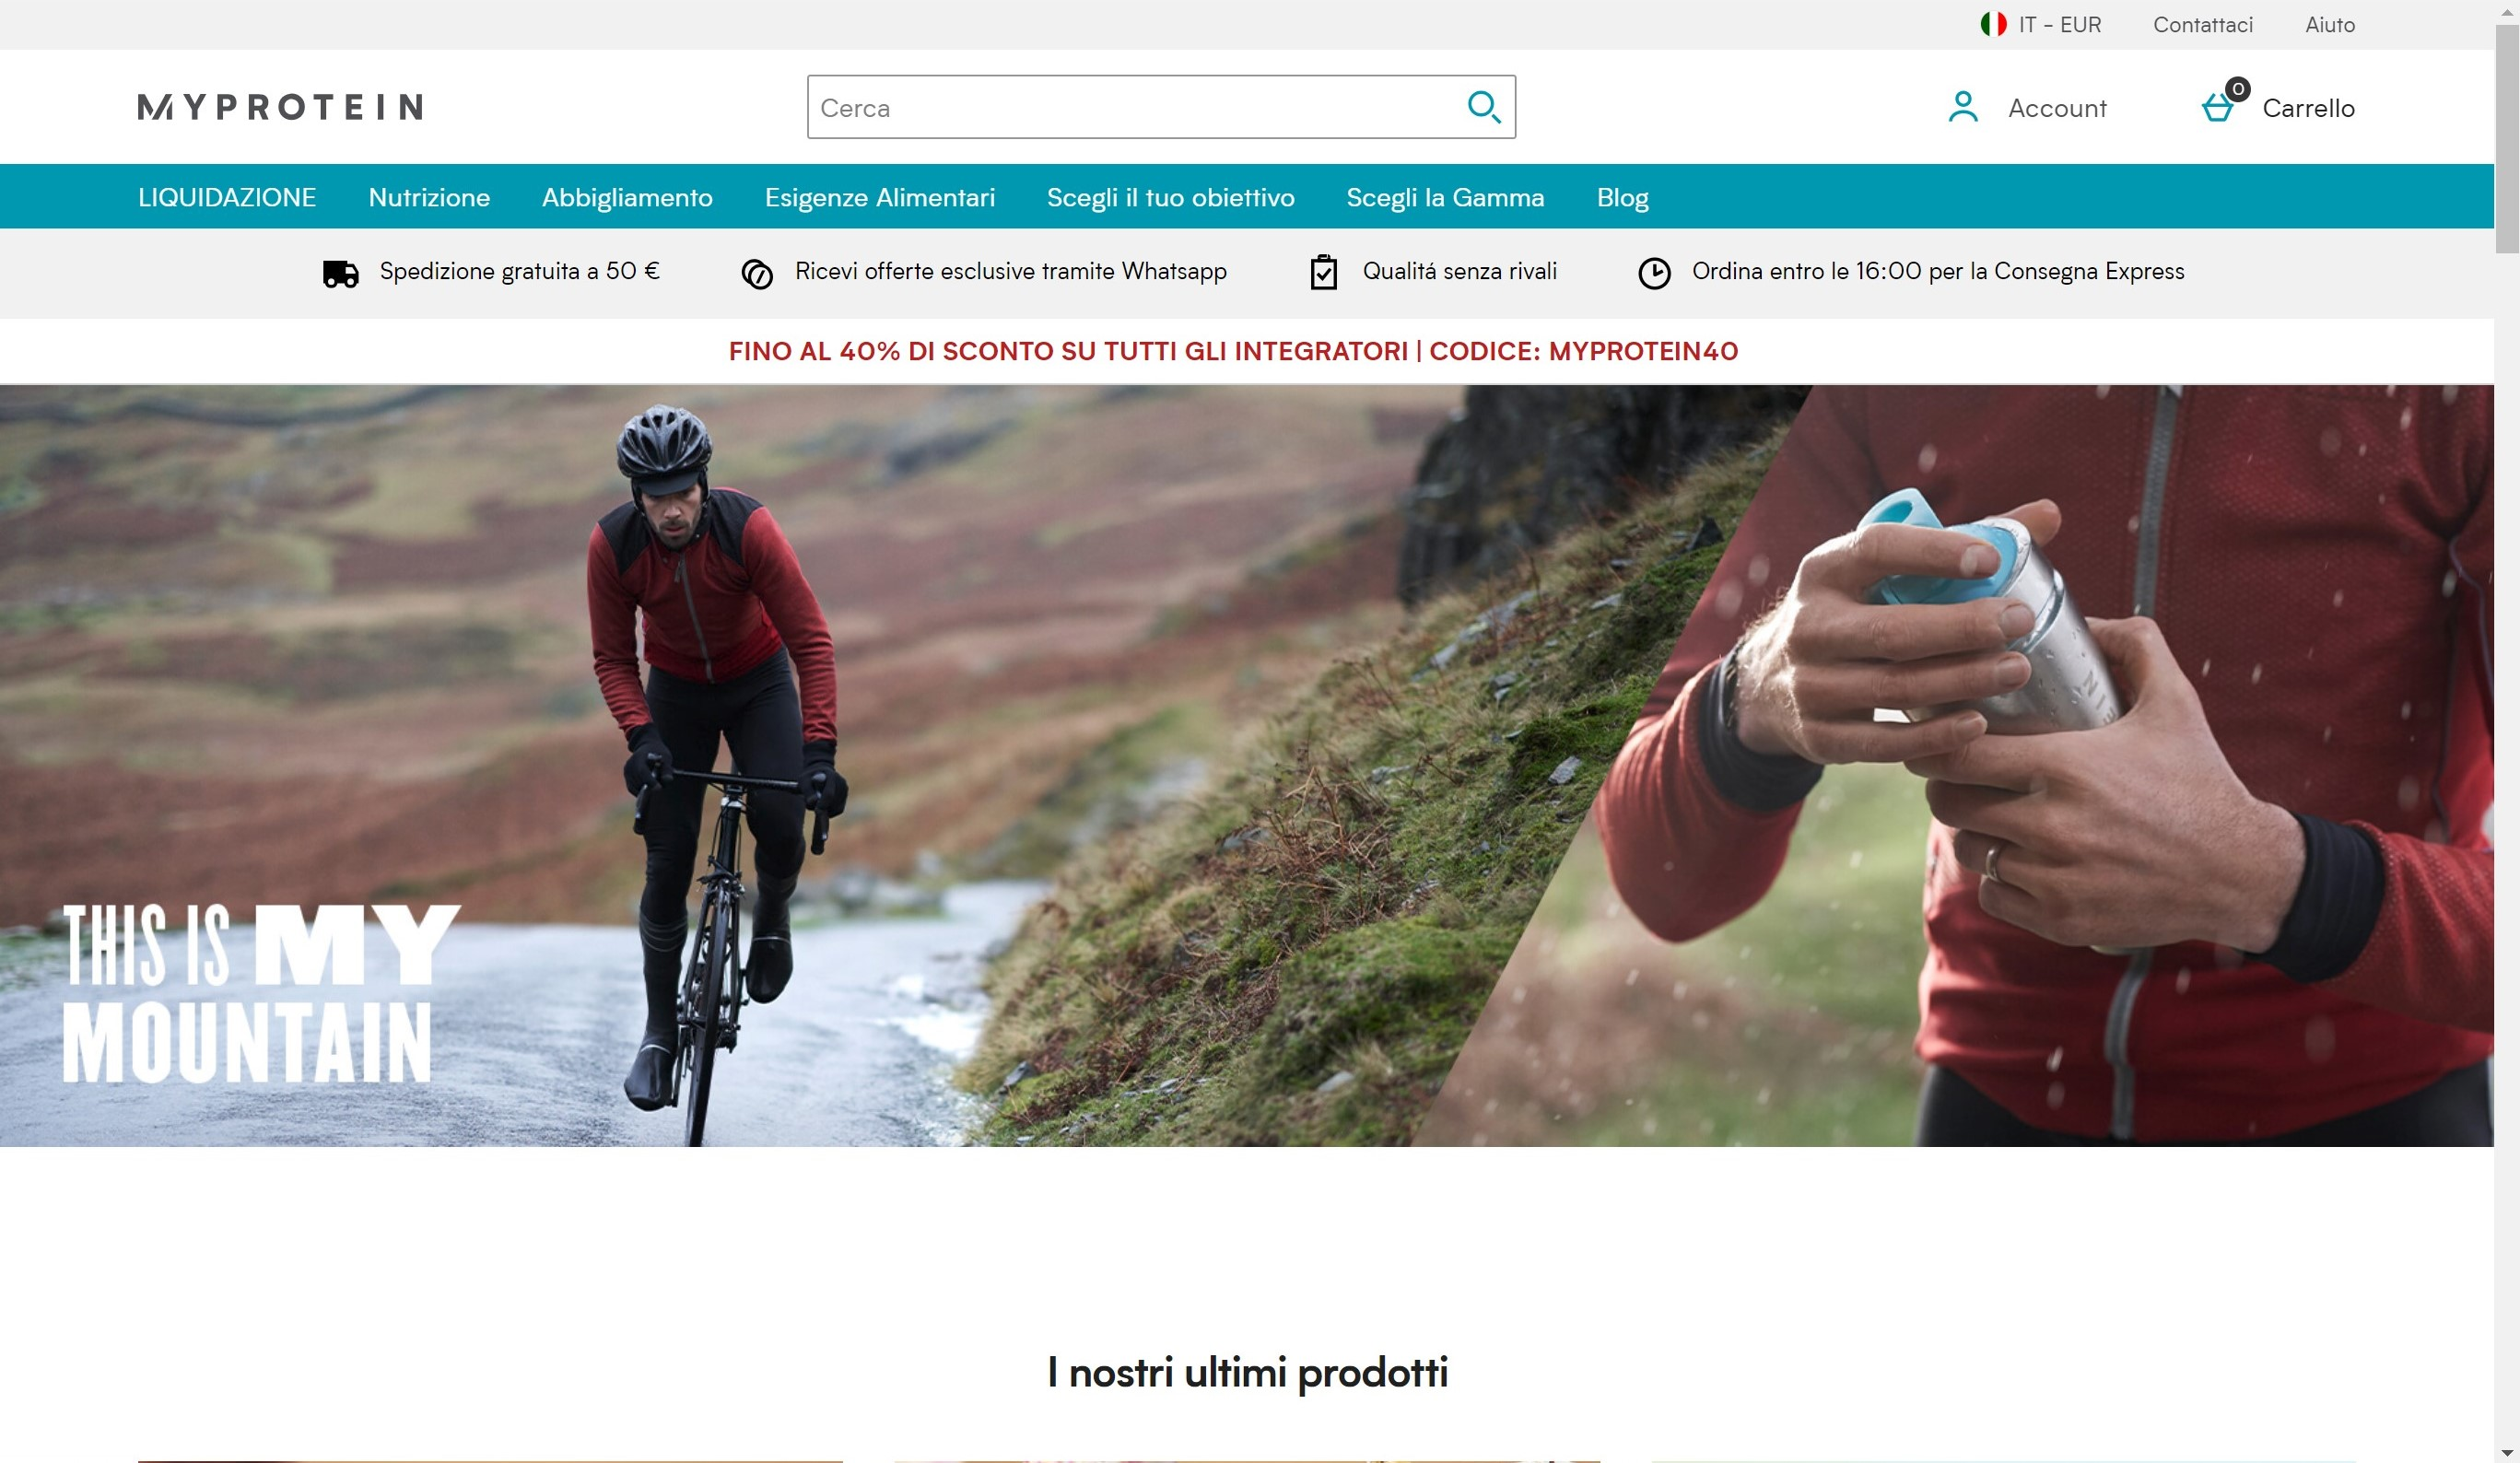
\includegraphics[width=\textwidth]
		{img/figura1.jpg}}
	\caption{\label{fig:figura1} Porzione visibile della homepage di MyProtein. Ho lasciato apposta visibile la scrollbar a destra per far capire quanto "alta" sia la pagina.}
\end{figure}
\subsection{6 Assi informativi}
La homepage è il luogo dove l'internauta cerca informazioni, che essa deve rendere disponibili nel modo migliore possibile. Fortunatamente questo problema trova un omologo nel giornalismo, in cui un articolo, pur avendo una quantità limitata di parole a disposizione (dettate dalle esigenze di impaginazione), deve poter fornire una descrizione completa dell'argomento affrontato, rispondendo a delle domande, le cosiddette 6W: \textit{Where, Who, Why, What, When, How}. Esse possono essere reinterpretate in ambito web con le modalità che analizzerò nei paragrafi sottostanti.
\paragraph{Where - A che tipo di sito sono arrivato?}
Le parole "Carrello" e "Spedizione gratuita sopra i 50 \euro" suggeriscono sito di e-commerce. Nome e menù suggeriscono che sono arrivato ad un sito che vende integratori proteici (prettamente) e anche abbigliamento (menu). 

\paragraph{Who - Chi c'è dietro al sito?}
Tutte le pagine del sito, quindi anche la Homepage, riportano nella parte alta (a sinistra o in centro, dipende dalle dimensioni dello schermo) il logo "MyProtein". Un problema è che al logo è associato il link alla homepage, e il collegamento alla pagina "Chi Siamo", contenente le informazioni sull'azienda dietro il marchio MyProtein, si trova nel footer del sito, a circa 4 o 5 scroll di distanza. Questo comporta, per l'utente, a capire istantaneamente di essere sul sito del brand MyProtein ma, se non conosce tale brand, potrebbe avere delle difficoltà nel capire chi è/cos'è MyProtein. Proporrei quindi uno slogan (magari sotto il logo), riassunto del seguente paragrafo di presentazione all'interno della pagina "Chi Siamo":
\begin{quote}
In quanto marchio leader nella nutrizione sportiva, forniamo una vasta gamma di prodotti di qualità tra cui proteine in polvere, vitamine, minerali, cibi proteici, alternative sane per la merenda e indumenti sportivi.
\end{quote}

\paragraph{Why - Perché dovrei dare la mia fiducia? Che benefici mi dà?}
MyProtein è un marchio molto famoso tra gli sportivi e gode di una fama molto positiva. In ogni caso, nella parte alta della homepage (sotto il menù), sono riportati i vantaggi che si ottengono comprando direttamente nel sito (si veda figura 2):
\begin{itemize}
	\item Spedizione gratuita per ordini di importo uguale o superiore a 50 \euro;
	\item Qualità dei prodotti;
	\item Possibilità di vedersi recapitare l'ordine il giorno successivo al pagamento (consegna express).
\end{itemize}
\begin{figure}[!htb]
	\center{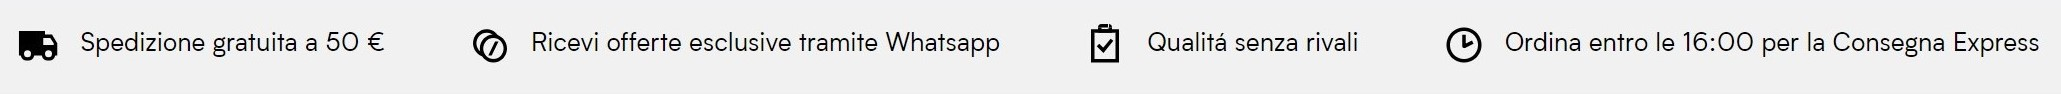
\includegraphics[width=\textwidth]
		{img/figura2.jpg}}
	\caption{\label{fig:figura2} Vantaggi di MyProtein, presenti in homepage}
\end{figure}
\paragraph{What - Che cosa offre il sito?}
Ancora una volta, il nome "MyProtein" suggerisce che i prodotti presenti nel sito abbiano qualcosa a che fare con gli integratori proteici. In ogni caso, le tipologie di prodotti offerti sono raggruppate in due categorie, "Nutrizione" e "Abbigliamento", che sono anche due delle voci del menù presente nella parte alta del sito. Inoltre, come specificherò meglio nel paragrafo successivo, nella homepage sono presenti alcuni prodotti in "esposizione", sebbene sia necessario quantomeno uno scroll per raggiungerli. Infine MyProtein possiede anche un blog (dove, tra l'altro, sono presenti numerose ricette "fit"), come si può evincere dall'ultima voce di menù.
\paragraph{When - Quali sono le ultime novità?}
Nella homepage sono due i punti principali in cui si possono vedere le ultime novità, in termini di prodotti/linee di prodotto o servizi:
\begin{enumerate}
	\item L'immagine larga nella parte centrale della prima porzione visibile (quella con la scritta "THIS IS MY MOUNTAIN" in bianco) indica generalmente l'ultima linea di prodotti inserita;
	\item Dopo una scroll è presente una sorta di vetrina delle novità in termini di prodotti (che, con fantasia, si intitola "I nostri ultimi prodotti"), riportata in figura 2.
\end{enumerate}
La soluzione adottata, a mio parere, è buona ma migliorabile: bisognerebbe ridurre l'enorme quanto inutile spazio verticale tra l'immagine di testata e la scritta "I nostri ultimi prodotti", che porterebbe la vetrina ad essere visibile (almeno parzialmente) senza dover scrollare.

\begin{figure}[!htb]
	\center{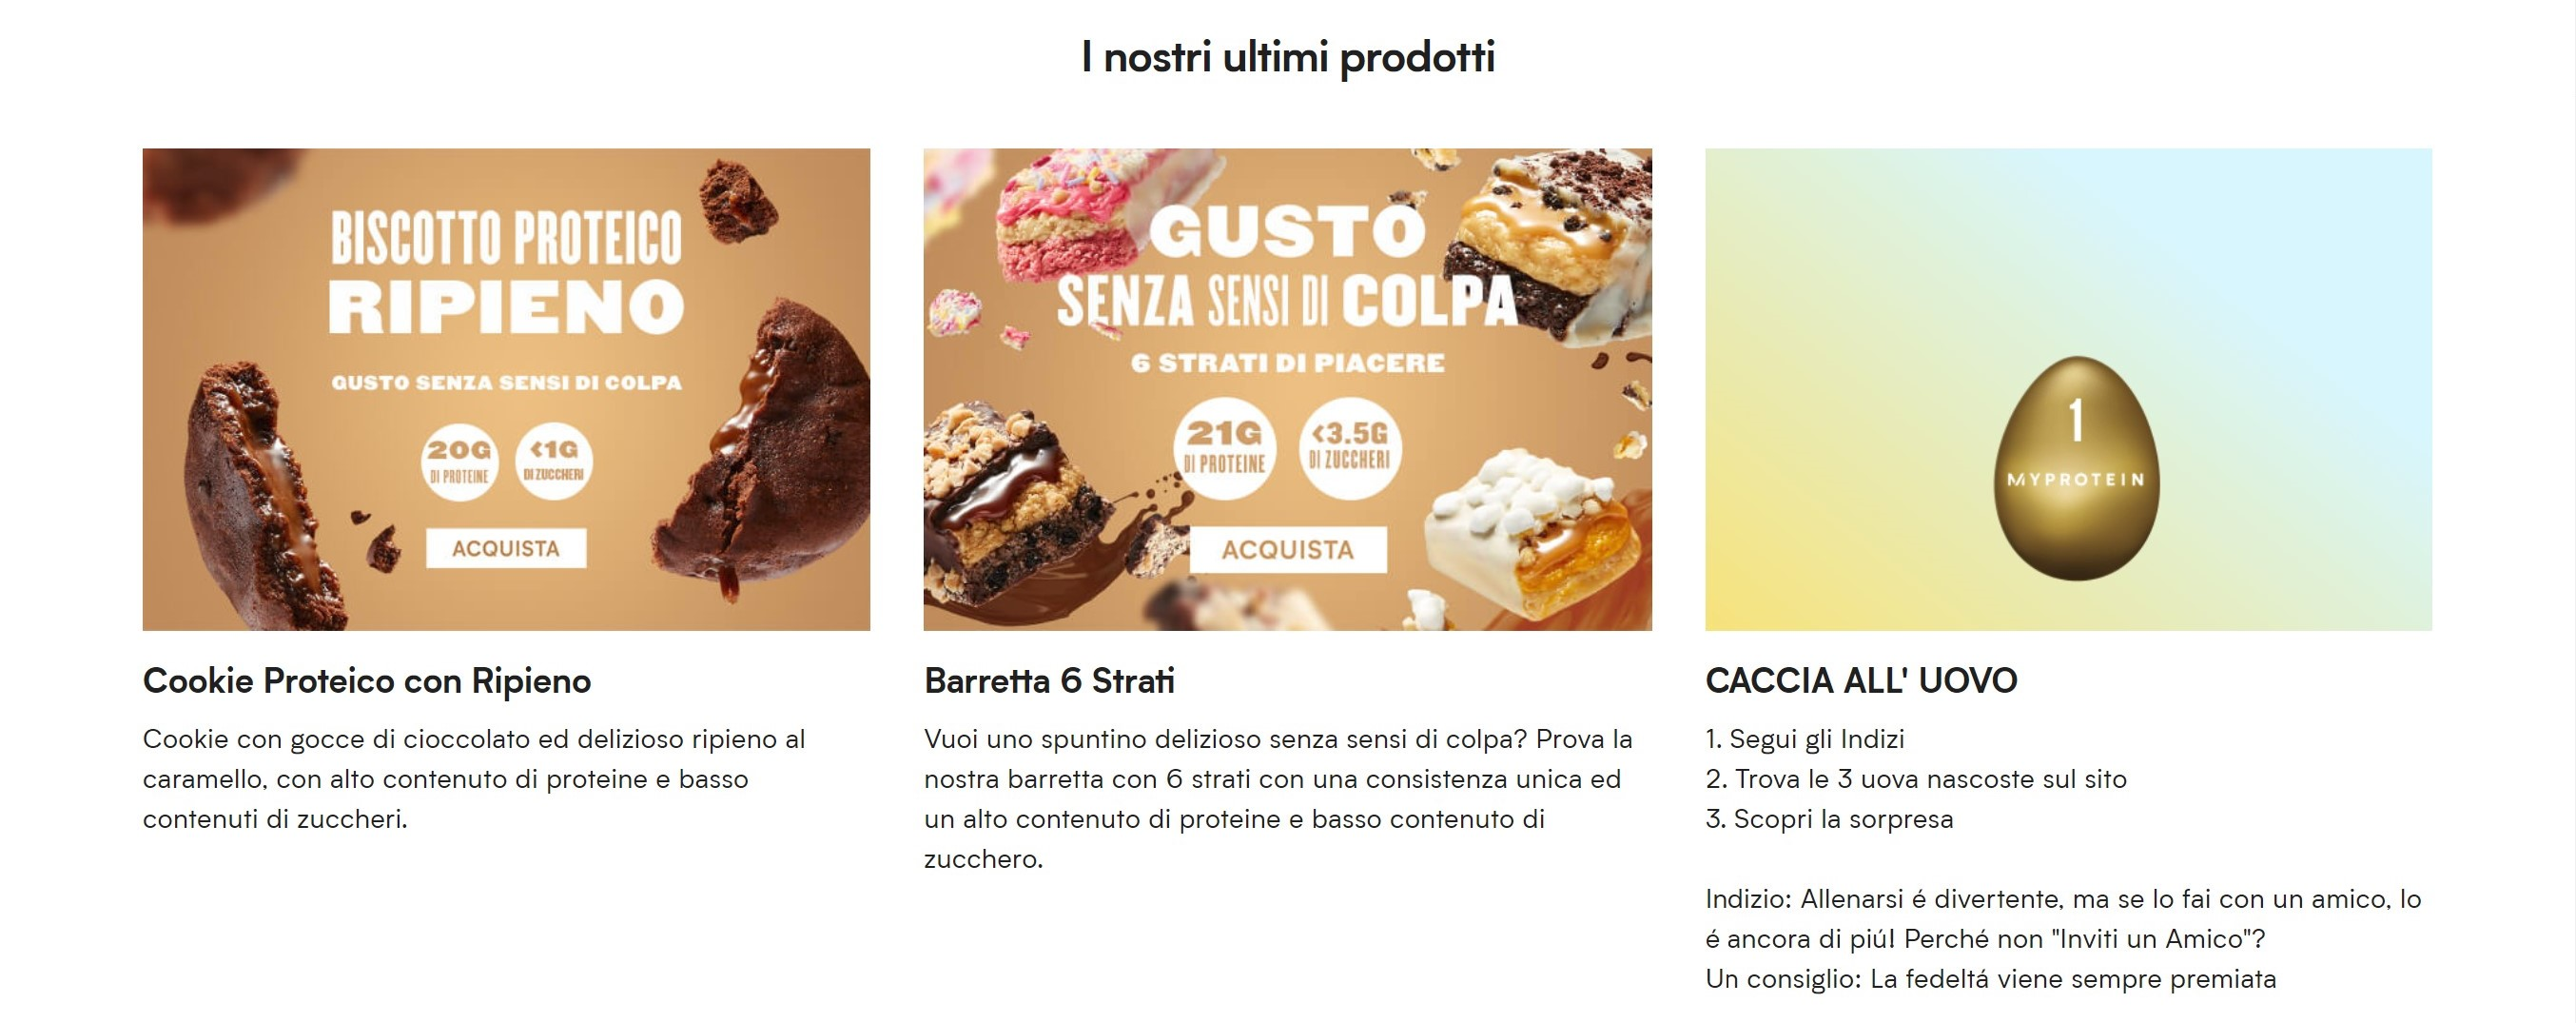
\includegraphics[width=\textwidth]
		{img/figura3.jpg}}
	\caption{\label{fig:figura3} Vetrina dei nuovi prodotti, presente in homepage}
\end{figure}
\paragraph{How - Come faccio a fare le cose?}
\label{paragraph:how}
A mio avviso, la navigazione all'interno del sito è abbastanza ben strutturata. Il menù di navigazione è diviso in sezioni: "LIQUIDAZIONE", "Nutrizione", "Abbigliamento", "Esigenze Alimentari", "Scegli il tuo obiettivo", "Scegli la gamma" e "Blog".
Cliccando o mettendo il mouse sopra una delle voci di menù, esclusa la prima e l'ultima, si accede ad un sottomenù a sua volta organizzato per argomenti. Prendendo l'esempio di "Nutrizione"  (visibile in figura 4), se a prima vista può sembrare un po' caotico, in realtà è molto ben organizzato e guida l'utente alla scoperta della gamma di prodotti, i quali adottano una catalogazione avanzata e "multi criterio", aiutando l'utente a trovare il prodotto giusto in base alle sue esigenze (come se fosse una ricerca guidata): prendendo l'esempio del prodotto "Impact Whey Isolate", esso appartiene sia alla categoria "proteine Whey" che a quella "Post Workout". \\Inoltre, nel caso si volesse trovare un prodotto specifico, è presente una barra di ricerca con tanto di anteprime e suggerimenti in tempo reale.\\L'unica nota negativa che ho trovato è la presenza di un altro menù nel footer del sito, in parte pure ridondante.
\begin{figure}[!htb]
	\center{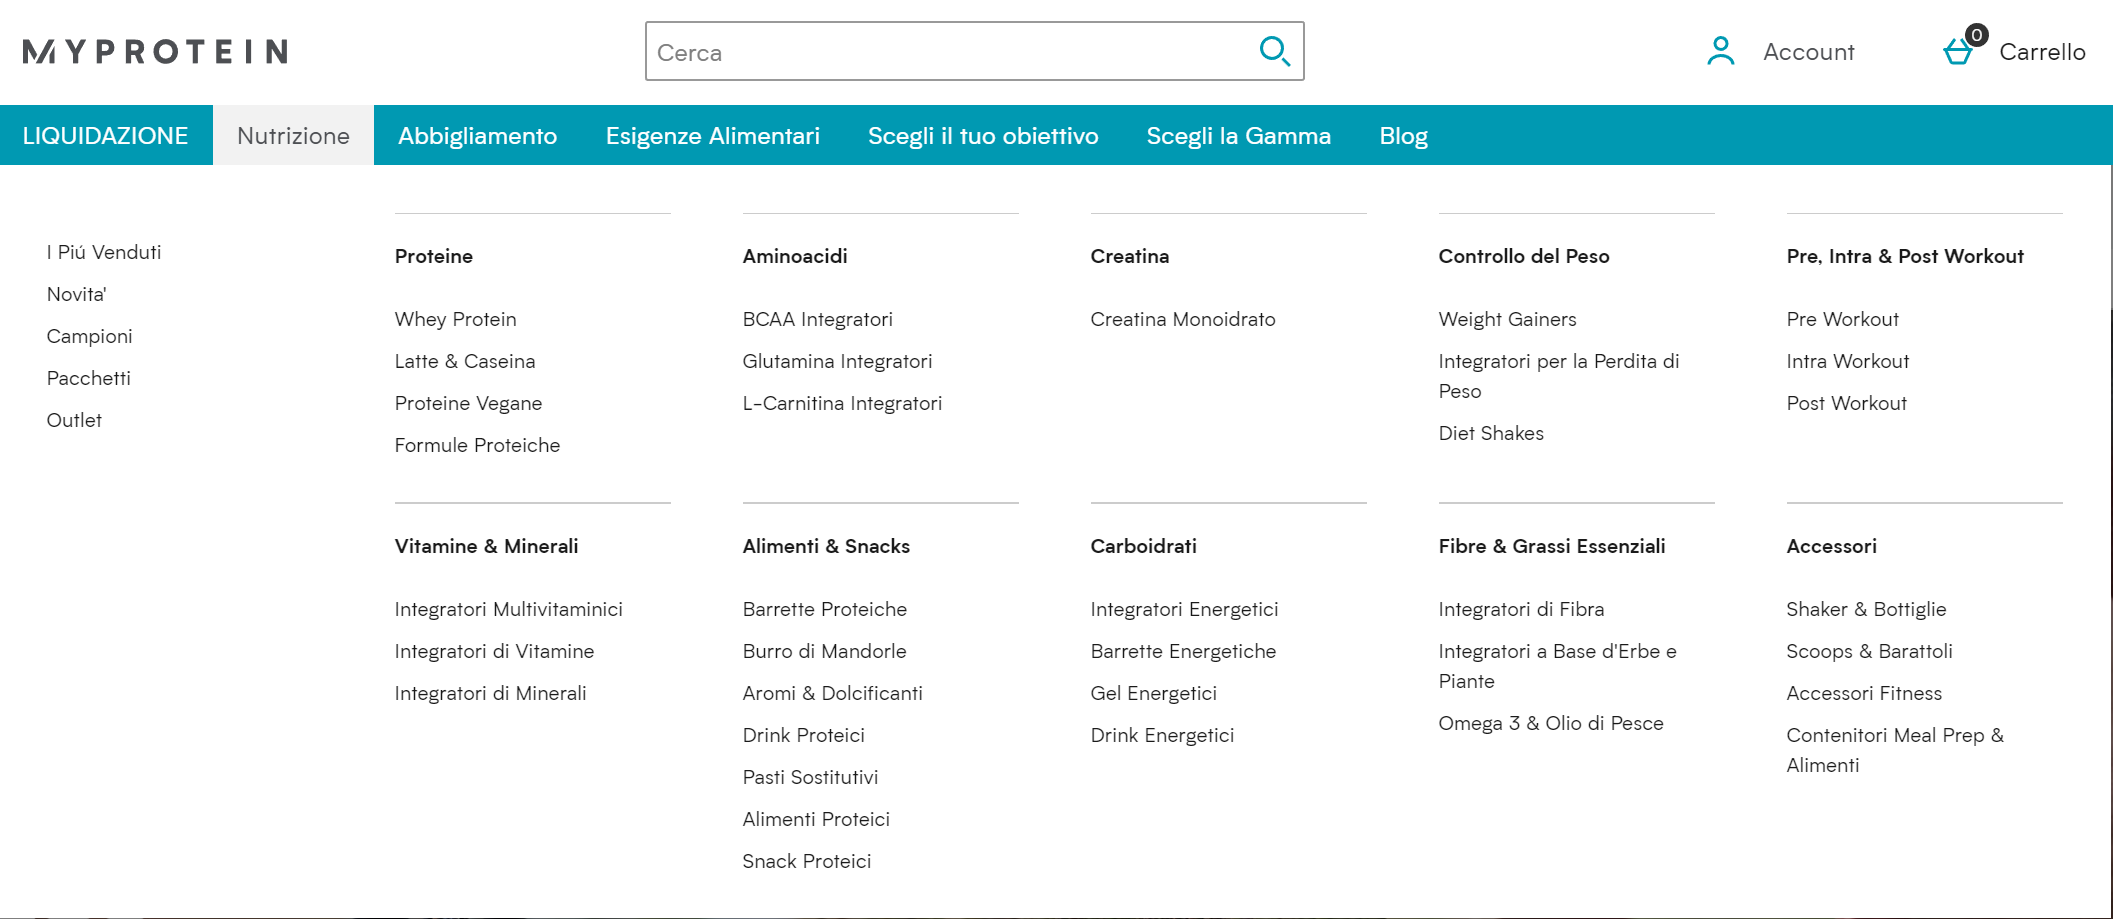
\includegraphics[width=\textwidth]
		{img/figura4.png}}
	\caption{\label{fig:figura4} Menù di navigazione e barra di ricerca}
\end{figure}
\subsection{I timer}
Il tempo che ci mette un utente a trovare un'informazione è molto importante. Se si considera che un visitatore dedica in media dai 31 ai 14 secondi alla sua ricerca: questo aspetto risulta molto importante nel determinare il successo o il fallimento di un sito web. In homepage l'utente si aspetta di trovare risposte a tutte le 6W, quantomeno se è alla prima visita a cui, per altro, dedica in media più tempo, ovvero 31 secondi. In questo tempo è in grado di leggere circa 91 parole, ma anche meno se si considera il tempo di rendering del layout. In ogni caso, nella porzione visibile, che, come spiegato nei paragrafi precedenti, consente di rispondere alle 6W, sono presenti circa una 50ina di parole, sufficienti a rispettare i timer del visitatore.